\documentclass[12pt]{article}

\usepackage[italian]{babel}
\usepackage{graphicx}
\usepackage{geometry}
\usepackage[T1]{fontenc}
\usepackage[utf8]{inputenc}

\geometry{a4paper, top=3cm, bottom=3cm, left=3.5cm, right=3.5cm}
\graphicspath{ {./resources/} }

\title{Un implementazione di un sistema antifurto con Arduino e Raspberry Pi}
\author{Lorenzo Mustich}

\begin{document}
	\maketitle
	
	\vfill
	\begin{figure}[h]
		\centering
		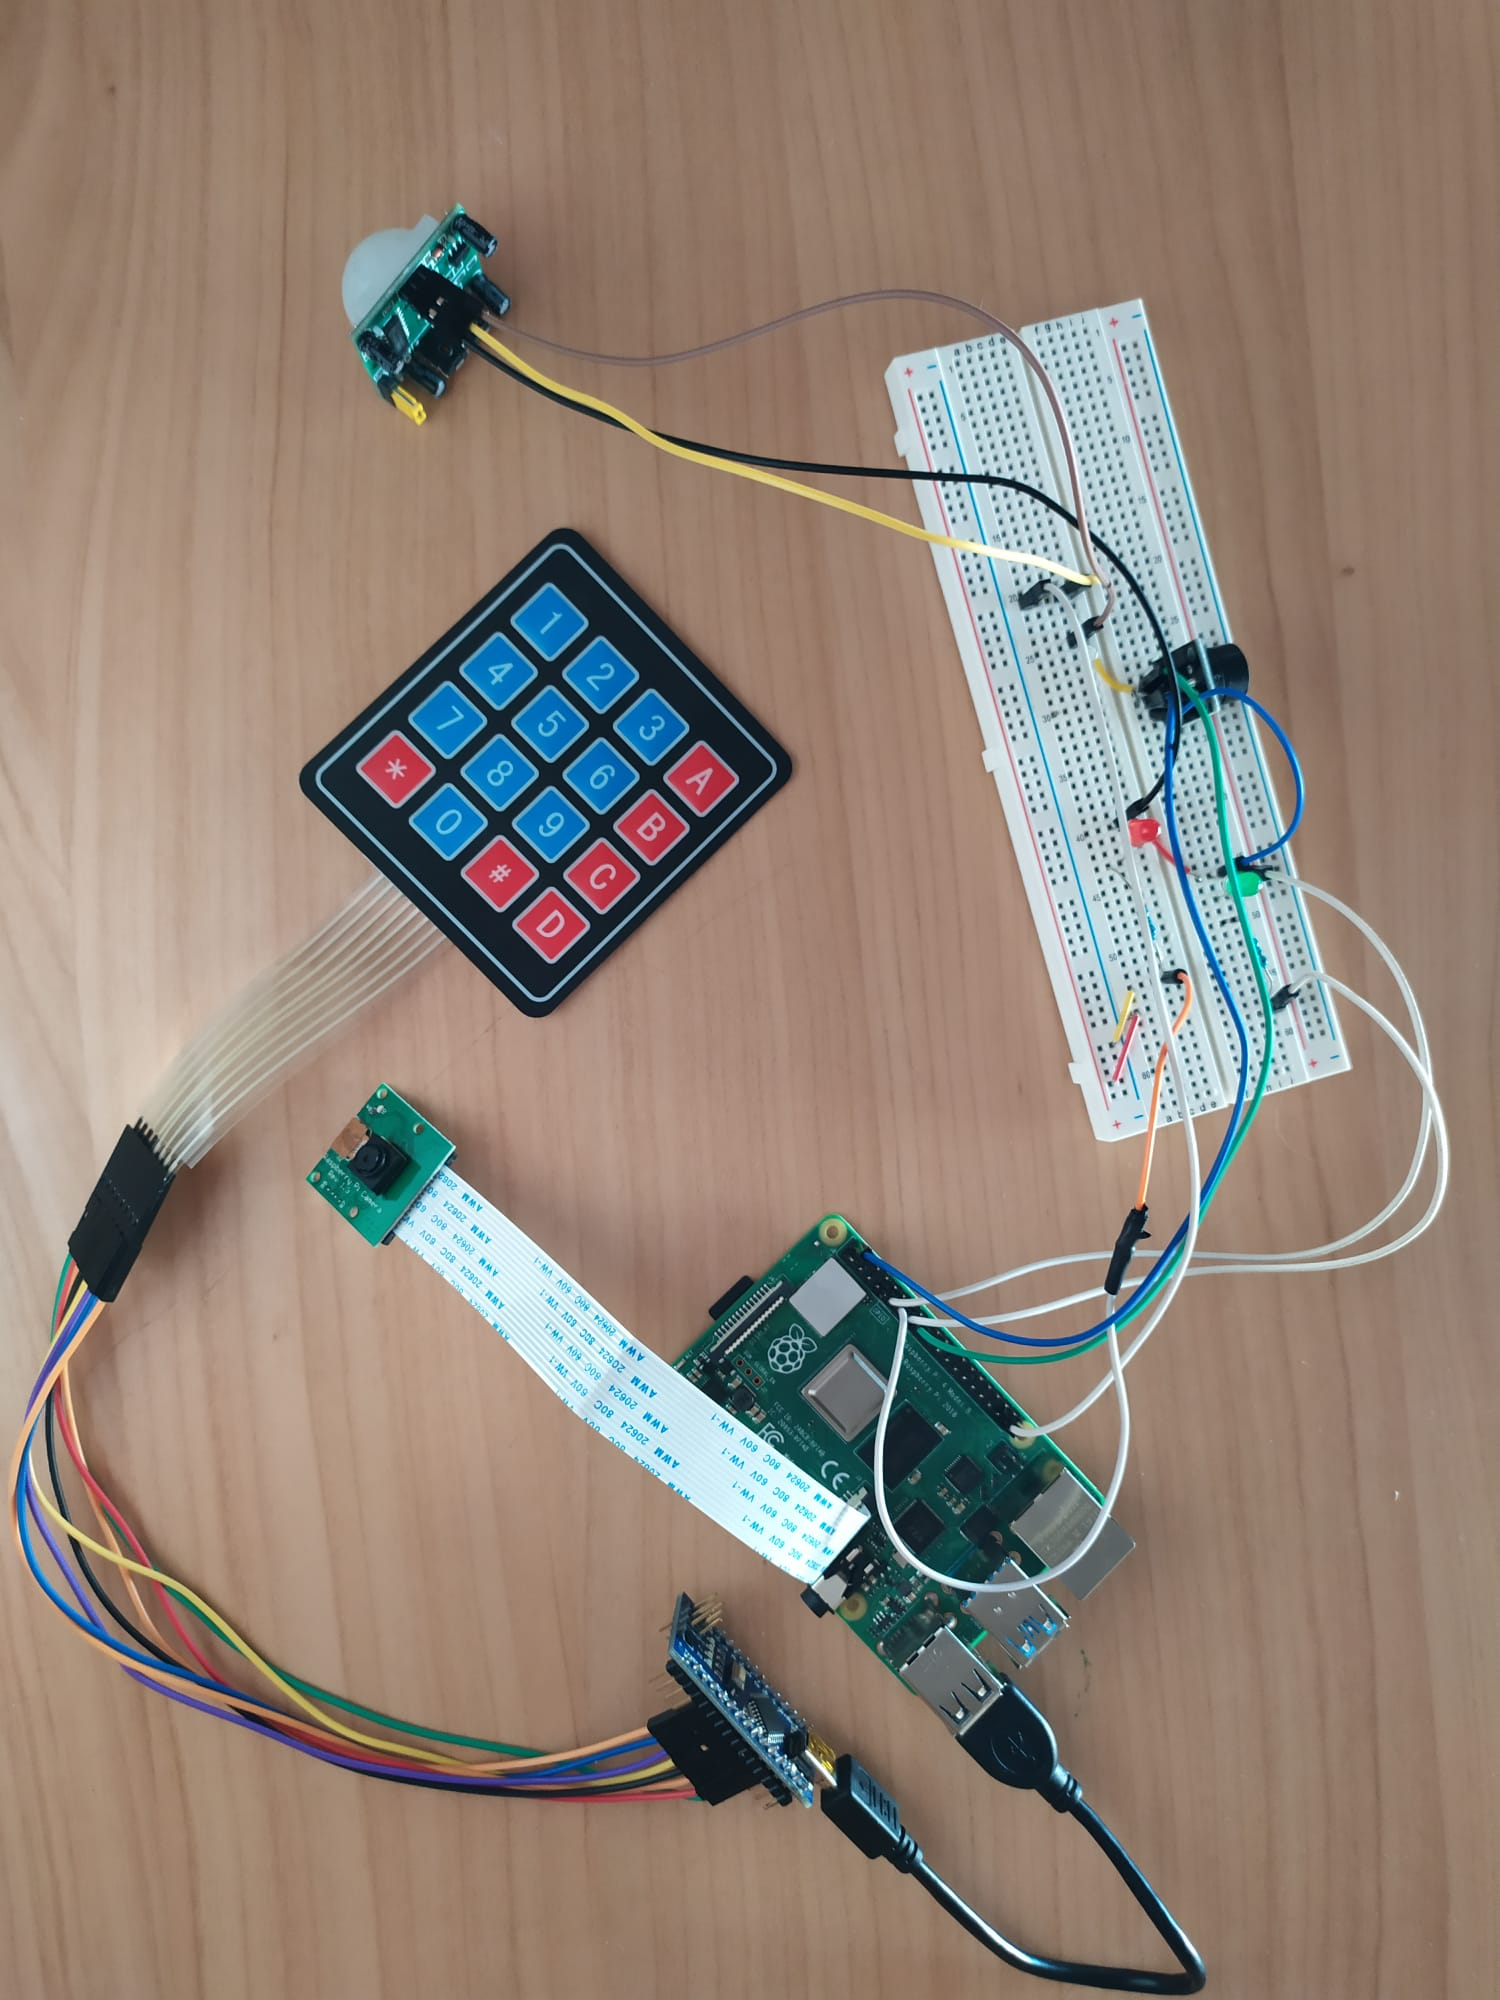
\includegraphics[width=4.0in]{prototipo}
	\end{figure}
	\vfill

	\pagenumbering{arabic}	

	\newpage
	\tableofcontents
	\newpage

	\section{Introduzione}
	Il progetto in questione tratta di un'antifurto da appartamento che utilizza un Raspberry Pi4 
	come unità centrale di elaborazione, un Arduino come controllo dell'input da utente e due bot 
	Telegram per l'attivazione e disattivazione e per l'invio dei video. 
	L'antifurto può essere attivato e disattivato in due modi: 
	\begin{itemize}
		\item utilizzando un bot scritto appositamente: \textbf{AntiTheftOnOff} 
		(\textbf{\textit{@ATOnOffBot}});
		\item nel caso in cui non si abbia la suddetta applicazione, digitando una serie di caratteri 
		alfanumerici per mezzo del tastierino a membrana.
	\end{itemize}
	Una volta attivato, un sensore PIR, appositamente tarato, rileverà eventuali movimenti 
	all'interno del suo campo visivo innescando l'accensione di una spia e di un allarme prodotto 
	da un buzzer attivo; successivamente, una videocamera produrrà un filmato di pochi secondi 
	dell'area. Un secondo bot Telegram (\textbf{ATVideoBot}, \textbf{\textit{@ATVideoBot}}) 
	è adibito all'invio del video al proprietario della casa. 
	\clearpage

	\section{Componenti}
	Di seguito è mostrata la lista dei componenti:
	\begin{itemize}
		\item Raspberry Pi4;
		\item Arduino;
		\item Sensori:	
		\begin{itemize}
			\item HC-SR501, sensore PIR di movimento;
			\item Buzzer attivo;
			\item PiCamera;
			\item Tastiera a membrana 4x4 16 tasti;
		\end{itemize}
		\item Led rosso/verde;
		\item Resistenze da ohm e da ohm
	\end{itemize}
	
	\begin{figure}[h]
		\centering
		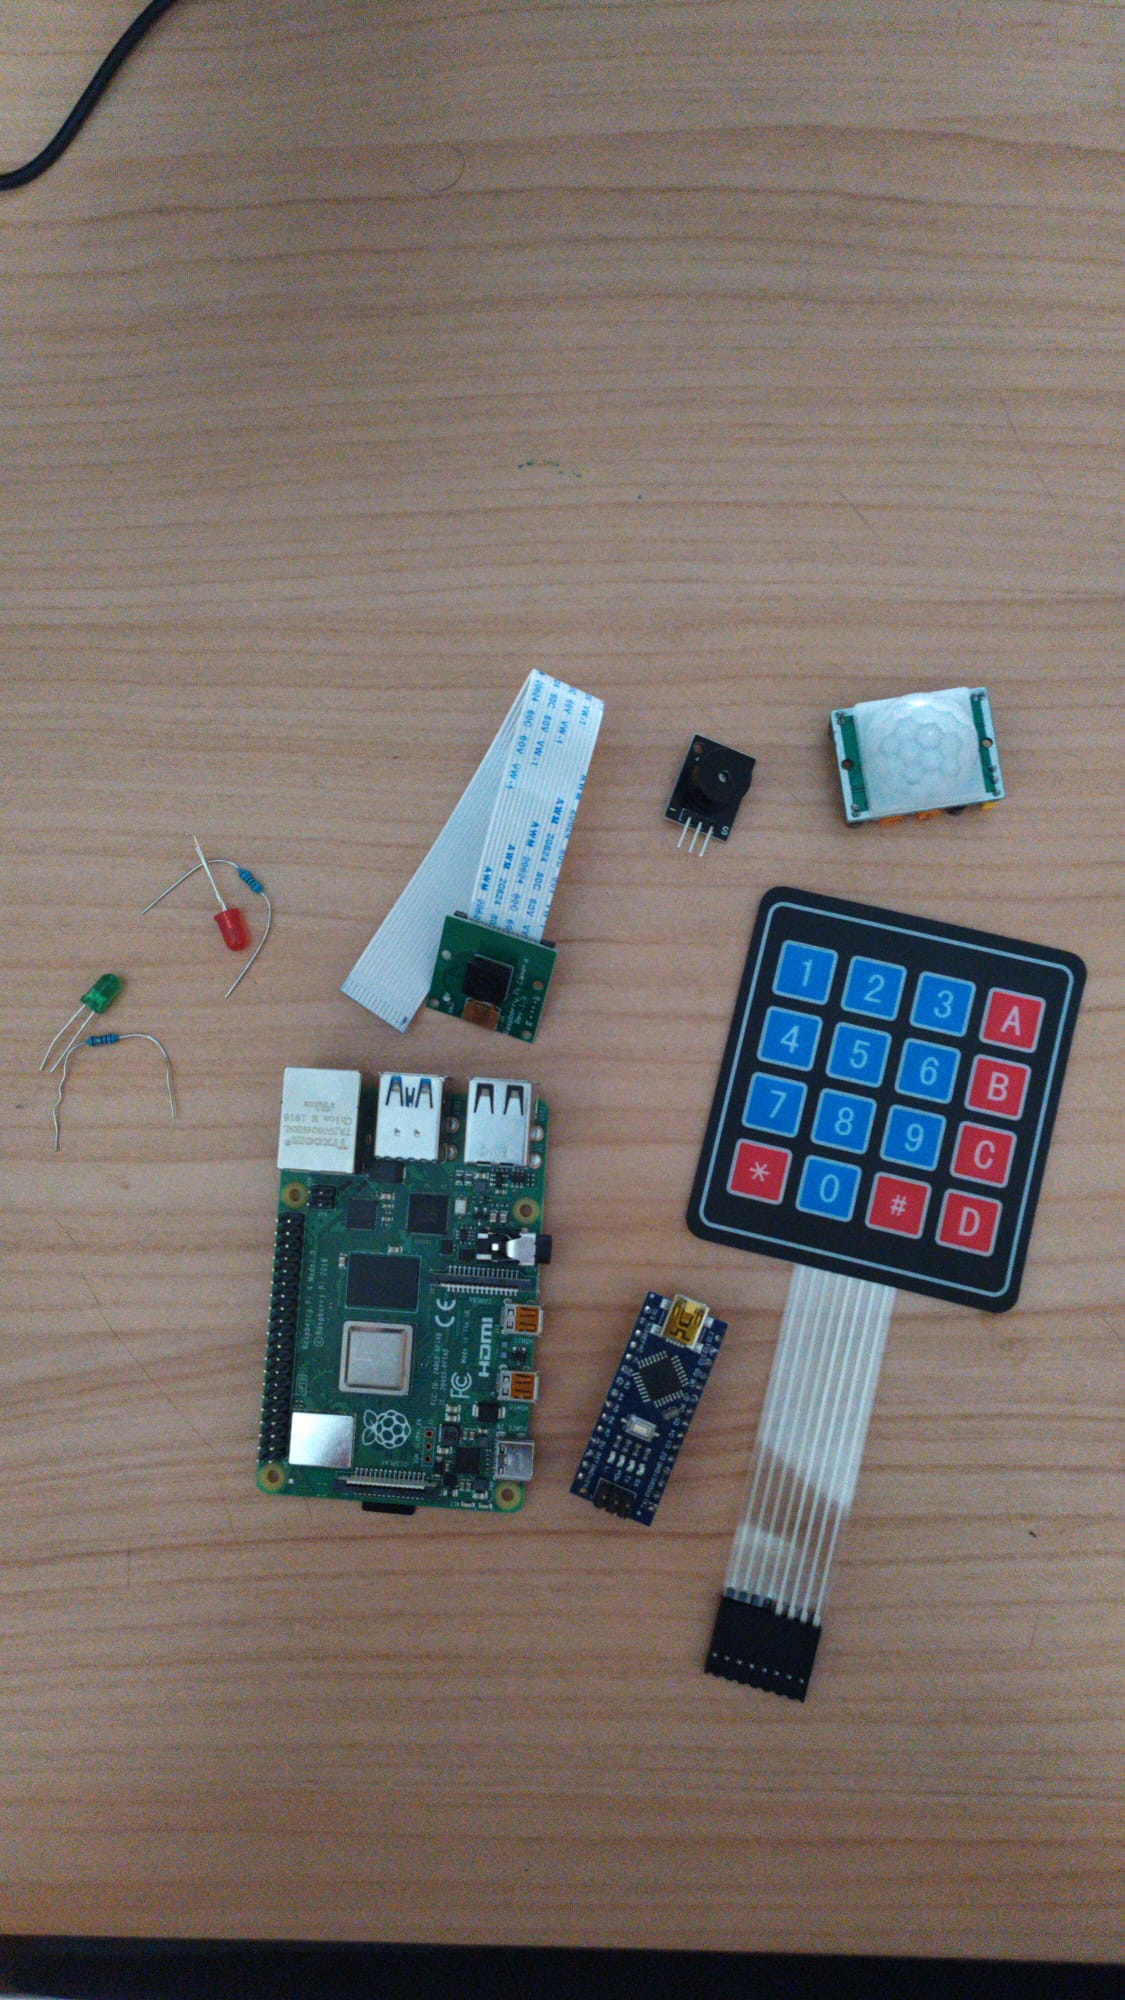
\includegraphics[width=2.0in]{componenti}
		\caption{Componenti del sistema}
	\end{figure}

	\subsection{HC-SR501 Sensore PIR}
	Si tratta di un sensore composto da due slot composte da un materiale sensibile agli infrarossi.
	Quando è in stato di \textit{idle}, i due slot captano la stessa quantità di raggi; 
	nel momento in cui un corpo caldo entra nella zona d'azione del sensore intercetterà il primo 
	dei due slot creando una differenza di potenziale all'interno del sensore. Quando il corpo lascia
	il campo visivo, esso intercetterà il secondo slot portando la differenza di potenziale ad un 
	valore negativo. Il sensore è in grado di rilevare questo cambiamento. Il 
	\textbf{sensore HC-SR501} ha un raggio d'azione di 110 gradi conici con una distanza che va dai 
	3 ai 7 metri.È possibile impostare per quanto tempo l'output del PIR deve essere tenuto alto dopo 
	la rilevazione del movimento: questo intervallo va dai 3 secondi ai 5 minuti.

	\section{Architettura}
	\begin{figure}[h]
		\centering
		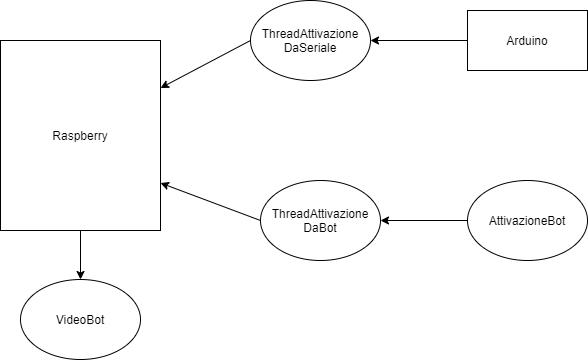
\includegraphics[width=3.0in]{architettura}
		\caption{Architettura del sistema}
	\end{figure}
	
	Raspberry ed Arduino comunicano tramite un cavo USB: alla pressione dei tasti corrispondenti 
	alla password viene scritto un carattere su seriale che viene recepito dal Raspberry, avviando 
	l'antifurto. Come spiegato precedentemente, l'attivazione può avvenire in due modi, 
	utilizzando un bot apposito o il tastierino a disposizione. Questi due metodi sono implementati 
	da due Thread che si occupano indipendentemente delle due modalità:
	\begin{itemize}
		\item nel primo caso, il microcontrollore confronta l'input da utente con la password scelta;
		\item nel secondo caso, l'utente invia dei comandi di attivazione e disattivazione tramite 
		bot.
	\end{itemize}
	Per notificare l'avvenuta accensione e spegnimento del sistema è stato posto un led rosso 
	lampeggiante.
	\newpage

	\section{Circuito}
	\begin{figure}[h]
		\centering
		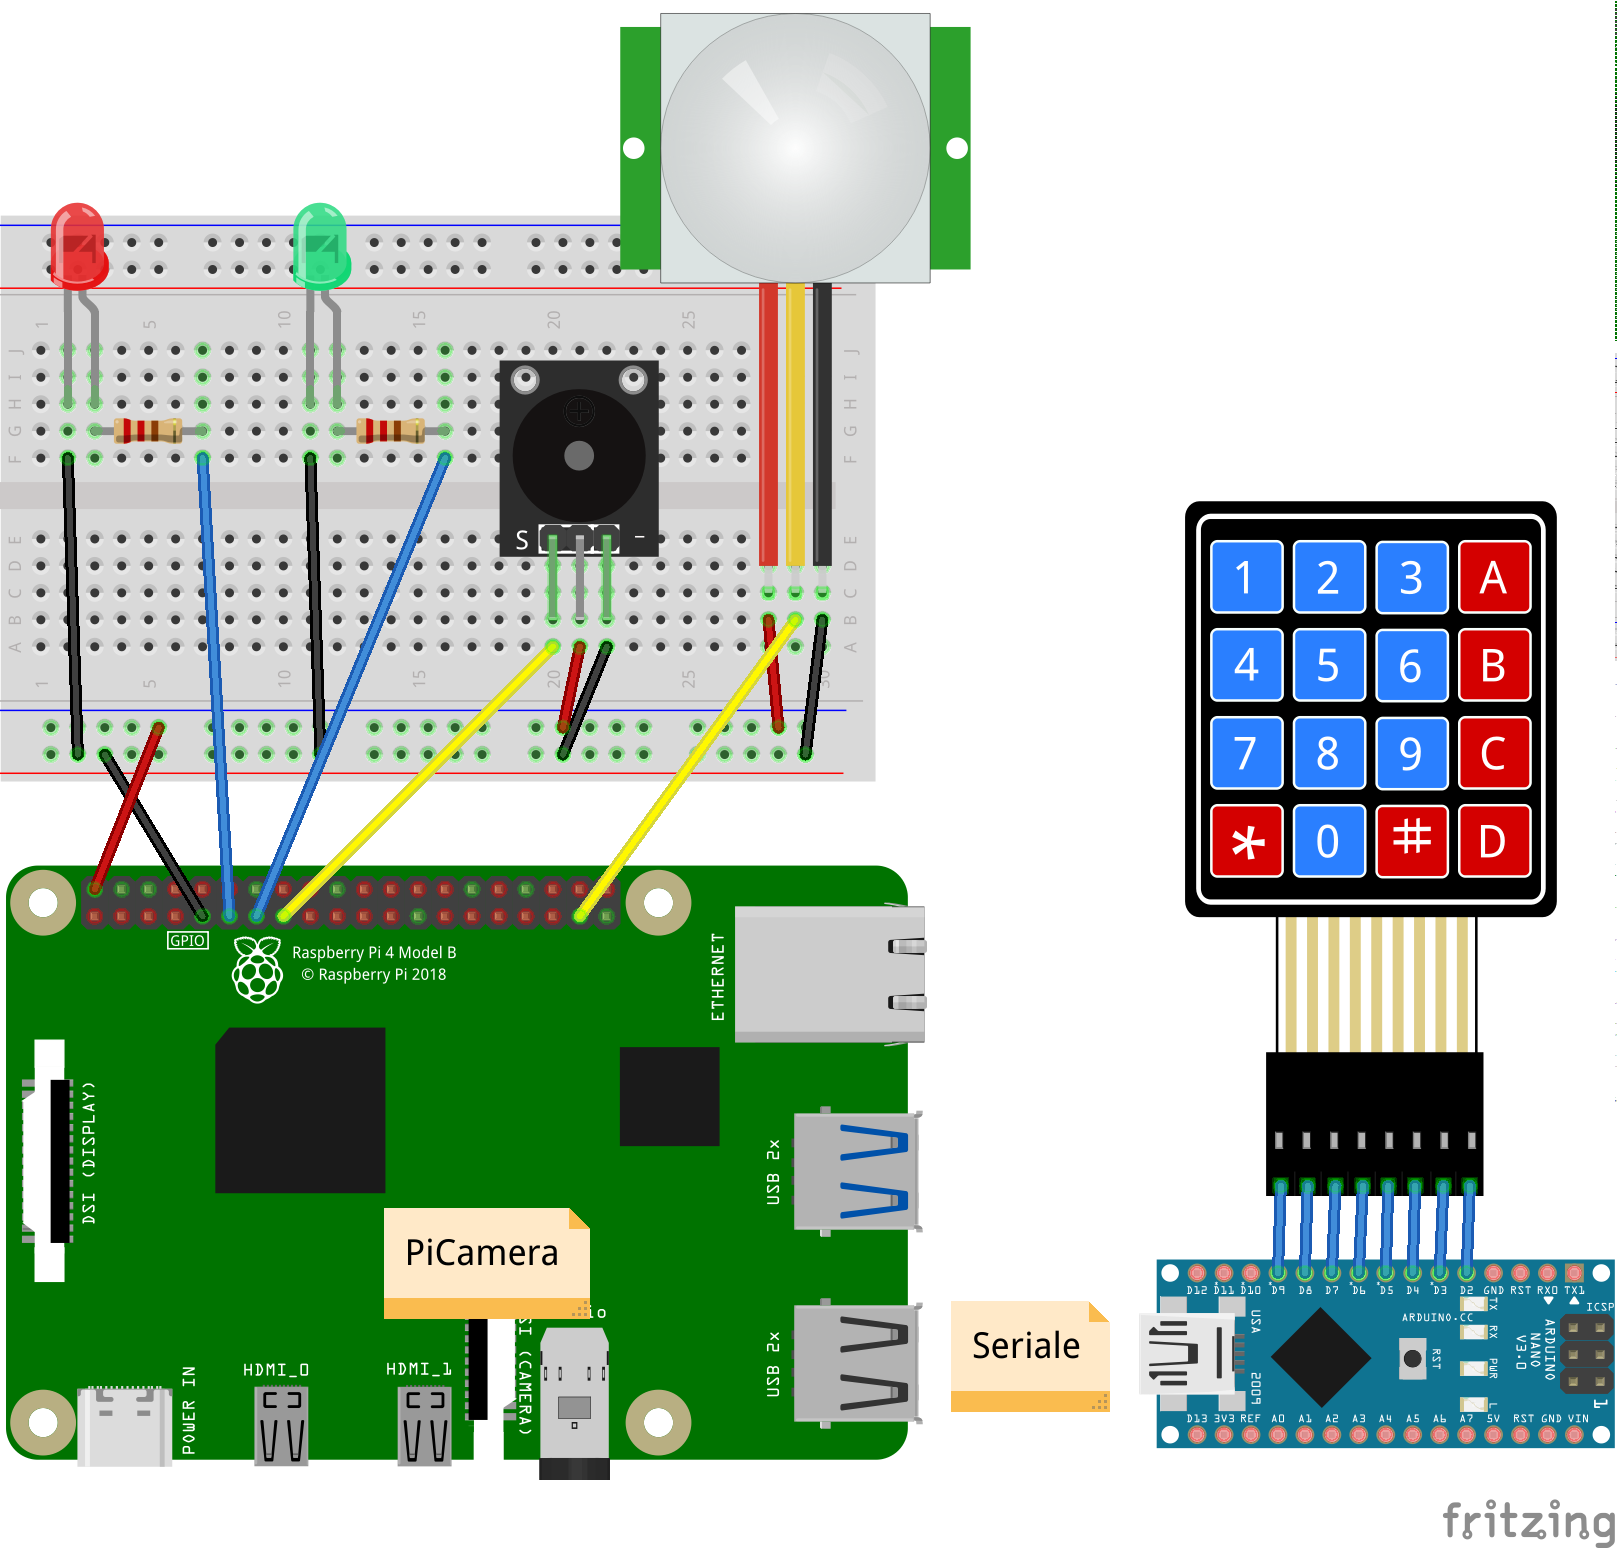
\includegraphics[width=4.5in]{circuito}
		\caption{Circuito}
	\end{figure}
	
	\section{Librerie}
	Ai fini del corretto funzionamento del sistema è necessario avere a disposizione le seguenti 
	librerie:
	\begin{itemize}
		\item Python (Raspberry Pi):
		\begin{itemize}
			\item modulo per bot Telegram: \textit{pip3 install python-telegram-bot};
			\item modulo per la gestione della camera: \textit{pip3 install picamera};
			\item modulo per la lettura da seriale: \textit{pip3 install pyserial};
			\item modulo per la conversione dei video: \textit{pip3 install ffmpeg-python};
		\end{itemize}
		\item Arduino:
		\begin{itemize}
			\item libreria Arduino per la gestione della tastiera: \textit{"Keypad.h"}
		\end{itemize}
	\end{itemize}

	\section{Conversione video}
	La PiCamera produce video in soli due formati, .h264 e .mjpeg, che non permettono la loro 
	fruizione da Telegram nella sua versione per smartphone. È stato necessario introdurre un 
	passaggio di conversione nel codice che permettese l'invio di file.mp4.

	\textit{ffmpeg -y -r 15 -i /home/pi/video.h264 -an -c:v copy /home/pi/video.mp4 > /dev/null > 2\&1}

	Di seguito la spiegazione dei vari parametri:
	\begin{itemize}
		\item -y: sovrascrive i file di output senza chiedere all'utente;
		\item -r: numero di fps;
		\item -i: percorso del file di input;
		\item -an: esclude dal flusso l'audio;
		\item -c:v copy: non effettua un nuovo encoding sul flusso video in uscita;
		\item -o: percorso del file di output
	\end{itemize}

\end{document}
